\documentclass[10pt,a4paper]{report}

\usepackage[utf8]{inputenc}
\usepackage{amsmath}
\usepackage{amsfonts}
\usepackage{amssymb}
\usepackage{graphicx}
\usepackage{listings}
\usepackage{hyperref}

\author{Diego A. Martinez Jimenez}
\title{Moogle}
\begin{document}

\maketitle

\begin{figure}
    \begin{center}
        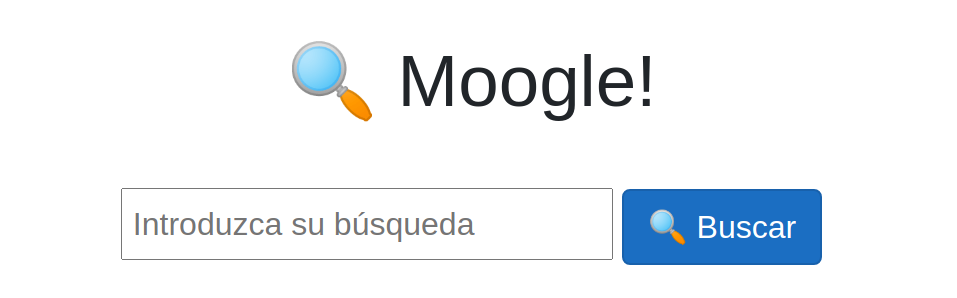
\includegraphics[width = 0.8\linewidth]{moogle.png}
    \end{center}
\end{figure}

\renewcommand{\thesection}{\arabic{section}}

\section{Instrucciones para correr el proyecto}

\textbf{Abrir una terminal en la carpeta del proyecto y escribir lo siguiente:}

\begin{itemize}
    \item Linux:
          \begin{itemize} \item \texttt{make dev} \end{itemize}
    \item Windows:
          \begin{itemize} \item \texttt{dotnet watch run --project MoogleServer}\end{itemize}
\end{itemize}

\section{Arquitectura del proyecto}

\begin{flushleft}

    Aceptando la mision que se me fue otorgada, ayude en la implementacion de \textbf{Moogle!}. Para ello tuve en cuenta la informacion que me pudieron proporcionar acerca de "\textbf{TF-IDF}" y "\textbf{Algebra lineal}". Tambien me fue util este link  \href{https://en.wikipedia.org/wiki/Tf%E2%80%93idf}{TF-IDF}

\end{flushleft}
    
\begin{figure}[h]
    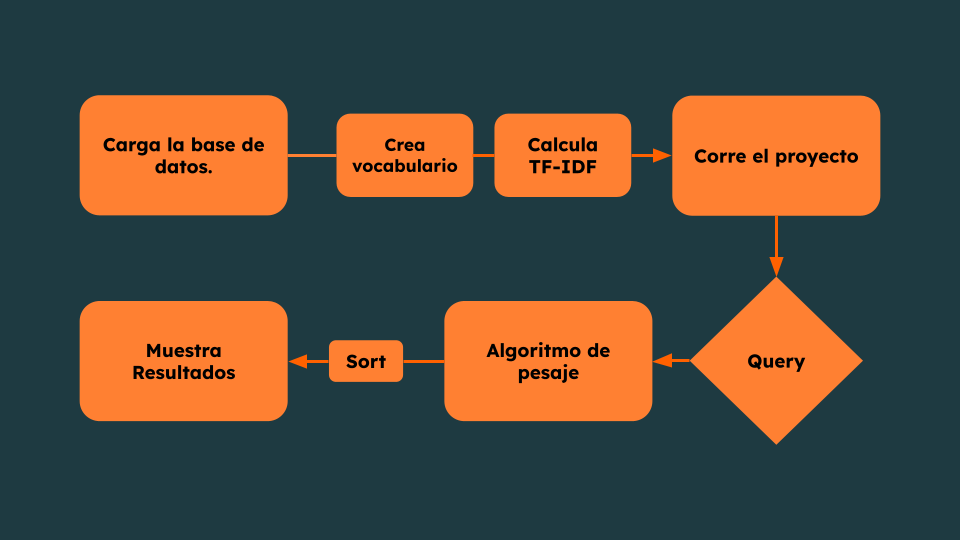
\includegraphics[width = 1\linewidth]{Project.png}
    \caption{Orden de los procesos del proyecto.}
\end{figure}

\subsection{Cargando la base de datos}

\begin{flushleft}

    Lo primero que implemente fue una clase que nombre \texttt{Documents} esta contiene varios metodos relacionados con operaciones que se le pueden a hacer a documentos, por ejemplo el metodo \texttt{Documents.ReadText()} el cual retorna como string toda el texto de un .txt. Lo mas importante de esta clase es su constructor:

\end{flushleft}

\begin{verbatim}
public Documents(string path){

        this.path = path;
        int documents = 0;
        
        this.directory = GetDocuments(this.path);
        this.Vocabulary = GetVocabulary();
        
        foreach( string file in this.directory)documents++;
        this.documents = documents;
        
        this.TF = new Matrix(this.documents,this.words);
        this.IDF = new Vector(new double[words]);
        _IDF = new Vector(new double[words]);

        this.ComputeDocuments();

        _TFIDF = this.TF;
        _Vocabulary = this.Vocabulary;
        Doc = this.directory;
}
\end{verbatim}

\begin{flushleft}

    Este recibe como parametro \texttt{string path} que debera ser un string con la direccion de una carpeta donde esten almacenados documentos \emph{.txt}, \textit{(de no ser asi no garantizo su correcto funcionamiento)}. Al crear una instancia de \texttt{Documents} esta asigna un numero a cada termino encontrado en el corpus, (el metodo encargado de este proceso es \texttt{Documents.GetVocabulary}) luego el metodo \texttt{ComputeDocuments} calcula el TF-IDF de cada documento, creando una matriz donde \texttt{TFIDF[i,j]} tiene guardado el TF-IDF de el termino j en el documento i. Toda la informacion util es almacenada en variables tipo \texttt{static} para su uso posterior.\\

    En las clases \texttt{Algebra.Vector} y \texttt{Algebra.Matrix} estan implementados en metodos las operaciones relacionadas con estos conceptos provenientes del \textbf{Algebra Lineal}. Estas son fundamentales para el funcioanmiento de \texttt{MoogleEngine.Documents}.

    \vspace{10pt}
    
    El TF-IDF se calcula a partir de las siguientes formulas, donde \emph{$f_{t,d}$} representa la cantidad de veces que aparece un termino \emph{t} en el documento \emph{d}, luego \emph{D} representa el corpus, es decir el conjunto de todos los documentos :

\end{flushleft}

\begin{center}
    \begin{large}
        $
        \mathrm{TF}(t,d) = \frac{f_{t,d}}{\max\{f_{t',d}:t' \in d\}}\hspace{20pt}
        \mathrm{IDF}(t,D) = \log \frac{N}{|\{d \in D: t \in d\}|}\linebreak
        $
        $
        \mathrm{TF\text{-}IDF}(t,d,D) = \mathrm{TF}(t,d) \cdot \mathrm{IDF}(t,D)
        $
    \end{large}
\end{center}

\section{Respondiendo la query}

\begin{flushleft}
    Luego de implementar estas clases, arregle la clase Moogle la cual en su momento no era muy util. El objetivo principal de esta clase es responder a la query a traves del metodo \texttt{Moogle.Query}. La idea para este metodo es modelar un vector en el que cada componente de este, sea el TF-IDF de cada termino que pertenezca al corpus de documentos. Luego hallar el coseno entre este vector y cada uno de los vectores creados a partir de los documentos.

    Primero guardo en variables el TF-IDF, el IDF y el vocabulario previamentes calculados al cargar los documentos.
\end{flushleft}

\begin{flushleft}
    \begin{verbatim}
        
Matrix TFIDF = Documents._TFIDF;
Vector idf = Documents._IDF;
Dictionary<string,int> vocabulary = Documents._Vocabulary;
    
    \end{verbatim}

    Luego calcula el TF-IDF de cada termino en la query, en caso de un termino de la query no encontrarse en vocabulary sera ignorado:

    \begin{verbatim}
        
tfidf = Documents.CalculateTF(query,vocabulary);

for(int i = 0; i < idf.Count; i++){
    tfidf[i] *= idf[i];
}

    \end{verbatim}

    Se almacena luego en \texttt{tfidf} que es una variable tipo \texttt{Algebra.Vector} para luego calcular el Producto Punto entre tfidf y  cada uno de los vectores construidos a partir de la matriz TFIDF en esta linea:

    \begin{verbatim}
        Vector currentDocTFIDF = new Vector(TFIDF,i);
    \end{verbatim}

    El Producto Punto se calcula con el metodo \texttt{Algebra.Vector.DotProduct} que hace pues exactamente lo que su nombre indica. Luego el resultado del calculo sera el score de su respectivo documento. Luego los documentos son ordenados con el metodo \texttt{Array.Sort} dependiendo de su respectivo score. En caso de que el score de un documento sea 0 es ignorado pues no tiene relevancia alguna con la query.

    Luego se construye un \texttt{SearchResult} a partir de esta informacion guardada en items.
    
    \begin{verbatim}
        return new SearchResult(items, suggestion);
    \end{verbatim}

    \subsection{Las Sugerencias}

    \begin{flushleft}
    
    Para las sugerencias use el algoritmo de \textbf{\href{https://es.wikipedia.org/wiki/Distancia_de_Levenshtein}{Distancia de Levenshtein}}. Este calcula de forma dinamica el número mínimo de operaciones requeridas para transformar una cadena de caracteres en otra. El metodo para esto es \texttt{Documents.EditDistance} .

    Al recibir una query la sugerencia se calcula dentro del metodo \texttt{Utils.Suggestion} que por cada termino guardado en vocabulary calcula su respectiva Distancia de Levenshtein con respecto a la query.

    En caso de que no se encuentre ningun termino relacionado con query, \texttt{Moogle.Query} retornara los documentos relacionados con la sugerencia.

    \end{flushleft}

\end{flushleft}

\end{document}